\section{On-path serialization}

Given the overhead of remote conflict resolution and the performance bottlenecks
associated with RDMA hardware serialization, this section discusses how an
on-path serializer can dramatically increase real-world performance
by alleviating both issues.  To ground our discussion, we address both in the
context of Clover, a state-of-the-art far memory system. First we describe how
to effectively do away with the need for most retries by ``fixing'' operations
issued with stale hints in flight.  Second, we show how we can leverage our
ability to rewrite RDMA requests after their ordering is determined to replace
expensive compare-and-swap requests with simple write verbs and rely upon the
semantics of RDMA RC queue pairs to provide serializability.  Additionally, we
can leverage this same functionality to multiplex independent operations across
multiple QP to improve scalability.

\subsection{System overview}

Any asynchronous data structure which allows for lockless reads and
writes must have a mechanism in place to resolve conflicts. When
memory is close, conflict resolution strategies can make many reads
and writes quickly; in the uncommon case of a conflict, the cost of
resolution is typically amortized by the unlikelihood of the conflict
itself. In the case of far memory the cost of a conflict is severe. In
contrast to opportunistic algorithms in a shared-cache architecture,
in a rack-scale disaggregated system conflicts can be detected at the
top-of-rack switch and resolved in the data path. Our solution,
\sword, leverages programmable ToR switches to allow developers with
knowledge of the disaggregated memory protocol to resolve conflicts
transparently in flight as the operations flow traverse the ToR.

\begin{figure}
\center
  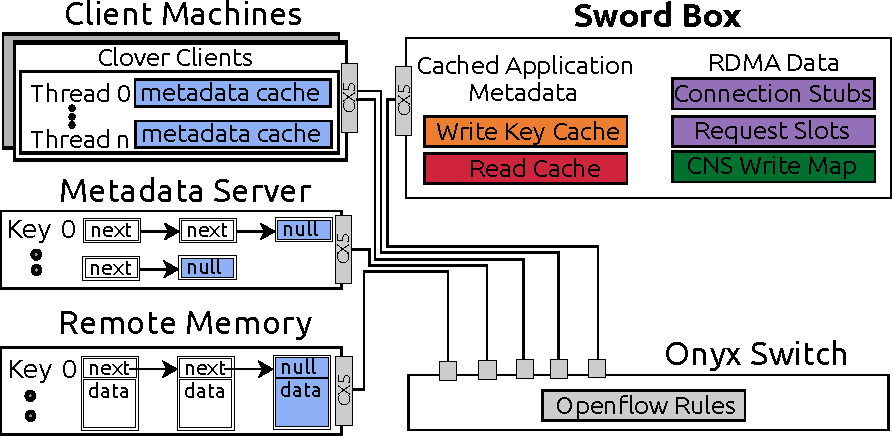
\includegraphics[width=0.45\textwidth]{fig/overview_2.pdf}
  %%
 \vskip 0.5em
\caption{Clients, Metadata and Remote Memory servers are
Clover components. {\sword} is run on a separate server connected to the same ToR.
Routing to {\sword} is effected by adding OpenFlow rules to redirect Clover traffic to \sword.}
%%
\label{fig:overview} \end{figure}

Figure~\ref{fig:overview} shows how {\sword} interacts with the Clover
system.  We envisage {\sword} implemented either as a part of or in-line with
a programmable switch that serves as the ToR switch
for all of the memory servers.  Client machines need not be directly
attached to the ToR, although they likely would be in most rack-scale
deployments.  Similarly, the topological location of Clover's metadata
server is irrelevant, but we expect it is also likely connected to the
same switch.  For the purposes of our discussion, we presume that
{\sword} first places all received RDMA requests into a total order
before processing them; likewise responses from a given 
server are totally ordered before processing.

\subsection{Conflict avoidance}

The single biggest impact an on-path serializer like {\sword} can have
is to dramatically decrease the likelihood of a failed RDMA request due
to a stale hint.  Specifically, because {\sword} can observe and
modify operations as they go by, it can ``correct'' any requests it
knows to be likely to fail.  Note that such replacement is strictly a
performance enhancement---because the requests continue to be
processed by the server as usual, any subsequent reordering will
cause the request to fail (and be retried by Clover), just as
it would have without rewriting.

\subsubsection{Write steering}

Recall that writes (committed with compare-and-swap requests) in
Clover are destined to the presumed tail of a key's linked list, but
the target of any individual RDMA request may be out of date due to
races with concurrent updates.  To prevent such requests from
failing, {\sword} maintains a cache of the location of the most-recent writes
for each key. If a write (CAS request) arrives at {\sword}
destined for a stale virtual address (i.e., an address other than the
one currently cached for that key), {\sword} replaces it with
the cached address.

While conceptually simple, the actual implementation is somewhat
involved due to the design of both Clover and the RDMA protocol and
our desire to remain transparent to both.  Specifically, Clover RDMA
CAS requests do not explicitly specify the operation of which they are
a part.  {\sword} infers the operation by checking the size of the
RDMA request and then extracts the key from the appropriate the
location in the packet.  The key is then used as an index into a
lookup table to find the virtual address of the latest write for that
key.  Our strategy requires only 64 bytes of data per key---the size
of the RDMA virtual address.  Because it modifies the content of the
RDMA request, {\sword} also needs to recompute the RDMA ICRC checksum
to prevent the server from rejecting the request as malformed.

%By
%performing this lookup in the data path all writes succeed regardless
%of how contested the memory address is. \todo{ref fig from words}.

\subsubsection{Read steering}

Reads present a slightly more complicated case. Writes contain the key
to which they pertain---which allows for a table lookup---but Clover's
RDMA read requests only contain the target virtual address and a size.
%When a
%read fails it must be retried, as mentioned earlier reads are
%performed iteratively until the tail of the list is reached, which in
%the case of highly contested keys could be arbitrarily long. Repeating
%reads does not destroy system performance as they are lockless,
%however in terms of client latency each retry adds serious
%latency. What makes handling reads hard is identifying the clover key
%for which the read is for, without additional data in the packet the
%value must be determined another way.
As reads can be for arbitrarily old virtual addresses a naive solution
that stored the lineage of each key would effectively require
caching the entire contents of Clover's metadata server.  Our solution
is to hash the address of each write into an array somewhat larger than
the size of the key space, and store the key along with the address.
Hash collisions are resolved by replacing the old address and key with
the new values, allowing keys with higher update rates to maintain
longer histories in the table. 

When reads arrive {\sword} looks up their destination address in the
table; if the address has a hit the associated key is used to look up
the current tail in the write cache and the RDMA read is redirected to
the cached location.  Should a miss occur---either because the hash
bucket was overwritten by another key, or because the tail address is
not cached---the read is left unmodified.  If it fails to arrive at
the current tail, Clover's default recovery mechanism kicks in and
performs a lookup to the metadata server for the last known address
and the process repeats. We find that by using an array size of
3$\times$ the vast majority of reads succeed first try. One advantage
of this technique is that it is a generalized cache for recent RDMA
reads, and requires little computation to maintain a hot cache. For
performance reasons we forgo heavyweight hash functions and use
the \texttt{murmur3} bit scrambler to attain an approximately even
hash of virtual addresses in only a few cycles.
%---which can likely be
%implemented on programable switch hardware.

\subsection{Enforcing ordering}

The combination of read and write steering dramatically improves the
performance of Clover (as shown in Section~\ref{s:results}), but only
scratches the surface of the potential improvements for far memory
systems.  In particular, if {\sword} is able to ensure that
requests will not be reordered between when it operates on them and
their arrival at a memory server---because, for example, it is
directly connected over a single link---we can leverage the ordering
semantics provided by RDMA queue pairs to completely eliminate data
races.  In that case, there is no need to incur the expense of RDMA
atomic requests; {\sword} can simply replace them with lightweight verbs
to dramatically increase the scalability of a given memory server.
Importantly, this optimization can be applied selectively to only the
set of servers (or keys) for which {\sword} is suitably located
and sufficiently provisioned to manage; Clover operations destined
for other servers and/or keys can be left unmodified---or subject just
to read/write steering as appropriate.

\subsubsection{Connection remapping}

Our key insight is that if all operations---across all client
connections---that share server state are vectored to the same queue
pair, RDMA's ordering semantics will provide sufficient serialization.
In general, the determination of which operations share state is
application specific and requires inspecting each packet, extracting
the relevant pieces of metadata, and vectoring the packet to the
correct connection.  In the particular case of Clover, it suffices to
identify RDMA requests that correspond to requests to read or write
the same key.

%%While removing locking operations is a general principle here we consider a
%%solution for RDMA.  %Different transports with different ordering guarantees
%%would require bespoke solutions.  

The challenge, of course, is that the RDMA specification stipulates
that each client establish its own queue pair with a given server, so
operations for a given key from different clients will arrive on
separate queue pairs.  \sword, then, must interpose on the
full set of queue pairs terminated by a given (set of) server(s) and
vector operations to queue pairs accordingly.

\paragraph{Sequence-space stitching.}

Multiplexing and demultiplexing RDMA requests across established
connections requires a significant amount of care. Requests on a
single connection must have monotonic sequence numbers from both the
sender's and receiver's perspectives. If monotonicity is broken, the
NIC will invoke an expensive go-back-$n$ protocol or issue explicit
congestion notifications. To ensure monotonic sequence numbers on
shared connections {\sword} tracks the outstanding sequence number per QP and
injects the appropriate sequence number into the packet after the
mapping decision has been made.  (Ironically, there is no need to
ensure any particular ordering among requests from separate clients, so
any total ordering suffices.)
%% This monotonic sequence number increment and QP mapping is the
%% serialization point which replaces the use of the RDMA CAS
%% request. As long as a packet is given an atomically incremental
%% sequence number from our middle box and placed on a stateful
%% partitioned connection, it will execute in the same serialized
%% order as if it were protected by a CAS. We are guaranteed this due
%% to the ordering requirements of RDMA reliable connections.

When an RDMA request arrives at {\sword} from a client, it is
mapped to the appropriate queue pair for the relevant key and a
\emph{stub} is stored to aid in mapping the request back, much like a
network address translator (NAT). The stub keeps track of the original
request's sequence number, IP address, MAC address, and queue
pair. Stubs are stored in an array of size $n$ indexed by their
sequence number$\pmod n$ to ensure $O(1)$ lookup when demultiplexing
the response.
%%
In addition to sequence numbers, a \emph{message} sequence number
is used as an RDMA optimization by the memory server NIC. This value
is transmitted as part of the RoCE BTH+ header in the response packet
and corresponds to the highest request number the server has
processed. If this value is wrong in the response packet from the
perspective of the sender (i.e., is less than another message sequence
number previously received by that client), the entire request is
retransmitted.  {\sword} maintains the message sequence number each client
expects to see by keeping track of the number of requests a client has
issued and adding it to the value of the original message sequence
number for that connection.

\paragraph{Request coalescing.}

As an additional complication, {\sword} must deal with the fact
that RoCE coalesces some ACKs as an optimization.  In particular
multiple RDMA requests can be acknowledged by a single
acknowledgment, in the form of either an ACK, ATOMIC ACK, or Read
Response. This occurs when multiple RDMA requests are processed
concurrently.  Because {\sword} maps requests across connections, some
coalesced acknowledgments may need to be disaggregated from the
clients' perspectives.
%
%A final additional challenge in mapping
%requests, is that receiving NICs can coalesce acknowledgment messages. Given a
%single connection, if two concurrent writes are issued, it is perfectly valid
%for an RDMA NIC to only ACK the second write. This is a challenge when mapping
%requests as a coalesced message might have been for a different sender. In our
%scheme as all requests have mapping stubs stored in the middle box,
{\sword} can detect such conditions by comparing the
acknowledged sequence number to that stored in a client's stub; when a
request is coalesced a gap in the sequence number is observable. In
this case we generate the needed acknowledgment at {\sword} and
insert it into the queue pair.
%While read, and CAS requests can not be
%coalesced, CAS requests mapped to writes can be. In the case of
%coalesced ATOMIC ACKs an atomic ACK is generated in place of the
%coalesced write ACK.



\subsubsection{Atomic replacement} 

Once any potentially conflicting operations are mapped to a single
queue pair, {\sword} is free to replace atomic requests such as
compare-and-swap with lightweight alternatives.  From a RoCEv2 perspective
the per-packet transformation from CAS to write can be applied easily
in the data path.  RoCEv2 CAS and write headers only differ by a few
fields. CAS can be thought of as a special case of a write, where the
write is conditional and the length is preset to 8 bytes.
%%

{\sword} transforms CAS requests to writes by modifying their headers: it
switches the RDMA OP field of the CAS to write, copies the CAS
value to the write payload location, sets the DMA length of the write
to 8, and shrinks the IPv4 length value by 4.  Post modification the RoCEv2
and IPv4 checksums are recalculated.
%so the modified packet will not be
%rejected by the memory side NIC.
The transformation from CAS to write
is deterministic and only requires a few cycles to transform the
header.

On the memory server, the NIC processes the write and responds with a
regular, write ACK. Once the ACK reaches {\sword} we apply the
inverse transformation from the ACK to an Atomic ACK which the sender
expects to see.  RDMA Atomic ACK headers are very similar to regular
ACKs with the only difference being that the atomic contains the
original data from the memory location of the CAS. This original data
is missing due to the transformation so we inject a value which
indicates success to the sender.
%%
This value is application specific; in Clover's case 64 zero bits
indicate success.  In other cases it may be necessary to store the
value in the request stub at {\sword}.

%Transforming CAS to
%write does nothing to disturb the RDMA protocol, as both the sender
%and receiver side NIC are oblivious.  However, the guarantees the
%atomic provides, such as write serialization and the prevention of
%read tearing has been lost. To prevent arbitrary corruption of data
%the serialization point must be placed somewhere else. Our approach is
%to detect conflicts in network, and utilize the in order delivery
%guarantees of RDMA reliable connections to ensure safe and serialized
%requests.


